\documentclass[a4paper,11pt]{article}
\usepackage[utf8]{inputenc}
\usepackage[T1]{fontenc}
\usepackage[french]{babel}
\usepackage[right=2.3cm, left=2.3cm, bottom=3cm, top=2.2cm]{geometry}
\usepackage[ddmmyyyy]{datetime}
\usepackage[table]{xcolor}
\usepackage{lmodern,mathptmx,changepage,titlesec,hyperref,listings,lstautogobble,graphicx,array,longtable,multirow,lipsum,tikz,shorttoc,enumitem,float,verbatim, amsthm,amsmath,amssymb,mathrsfs,thmtools}
\usetikzlibrary{arrows,automata}
\usetikzlibrary{positioning}

\renewcommand{\rmdefault}{\sfdefault} %Utilisation de la police sans-serif ("Computer Modern Sans") pour la police roman
\renewcommand{\ttdefault}{pcr} 	%Utilisation d'une police "CourrierNew" pour la police monospaced (pour faire un listing manuel)
\linespread{1.15}				%Interligne

%Utilisation de liens colorés en bleu et soulignés
\hypersetup{colorlinks=true, urlcolor=blue, urlbordercolor=blue, linkcolor=black, linkbordercolor=white}
\makeatletter \Hy@AtBeginDocument{\def\@pdfborder{0 0 1} \def\@pdfborderstyle{/S/U/W 1}}\makeatother

\titlespacing*{\section} {0cm}{7ex plus 1ex minus .2ex}{1.5ex plus .2ex}
\titlespacing*{\subsection} {0cm}{4.5ex plus 1ex minus .2ex}{1.5ex plus .2ex}
\titleformat*{\section}{\LARGE\bfseries}
\titleformat*{\subsection}{\Large\bfseries}
\titleformat*{\subsubsection}{\normalsize\bfseries}

\definecolor{darkgreen}{rgb}{0,0.8,0}
\definecolor{mygray}{rgb}{0.93,0.93,0.93}
\definecolor{mymauve}{rgb}{0.58,0,0.82}
\lstset{	
	language=C,
	captionpos=b,
	basicstyle=\small\ttfamily,
	backgroundcolor=\color{mygray},
	breaklines=true,
	breakatwhitespace=true,
	tabsize=3,
	frame=none,
	rulecolor=\color{black},
	keywordstyle=\color{blue}\bfseries,
	stringstyle=\color{orange},
	showstringspaces=false,
	commentstyle=\footnotesize\color{darkgreen},
	keepspaces=true,
	extendedchars=true,
	numbers=left,
	numberstyle=\tiny\color{lightgray},
	stepnumber=1,
	escapeinside={(@}{@)},
	autogobble=true,
	literate=
		{á}{{\'a}}1 {é}{{\'e}}1 {í}{{}}1 {ó}{{\'o}}1 {ú}{{\'u}}1
		{Á}{{\'A}}1 {É}{{\'E}}1 {Í}{{\'I}}1 {Ó}{{\'O}}1 {Ú}{{\'U}}1
		{à}{{\`a}}1 {è}{{\`e}}1 {ì}{{\`i}}1 {ò}{{\`o}}1 {ù}{{\`u}}1
		{À}{{\`A}}1 {È}{{\'E}}1 {Ì}{{\`I}}1 {Ò}{{\`O}}1 {Ù}{{\`U}}1
		{ä}{{\"a}}1 {ë}{{\"e}}1 {ï}{{\"i}}1 {ö}{{\"o}}1 {ü}{{\"u}}1
		{Ä}{{\"A}}1 {Ë}{{\"E}}1 {Ï}{{\"I}}1 {Ö}{{\"O}}1 {Ü}{{\"U}}1
		{â}{{\^a}}1 {ê}{{\^e}}1 {î}{{\^i}}1 {ô}{{\^o}}1 {û}{{\^u}}1
		{Â}{{\^A}}1 {Ê}{{\^E}}1 {Î}{{\^I}}1 {Ô}{{\^O}}1 {Û}{{\^U}}1
		{œ}{{\oe}}1 {Œ}{{\OE}}1 {æ}{{\ae}}1 {Æ}{{\AE}}1 {ß}{{\ss}}1
		{ç}{{\c c}}1 {Ç}{{\c C}}1 {ø}{{\o}}1 {å}{{\r a}}1 {Å}{{\r A}}1
		{€}{{e}}1 {£}{{\pounds}}1 {«}{{\guillemotleft}}1
		{»}{{\guillemotright}}1 {ñ}{{\~n}}1 {Ñ}{{\~N}}1 {¿}{{?`}}1
}

%Redéfinition de la taille de \Huge pour le titre du document
\makeatletter\renewcommand\Huge{\@setfontsize\Huge{32pt}{40}}\makeatother
\date{\today}

%\usepackage[french,frenchkw,ruled,vlined]{algorithm2e}

\title{\vspace{\fill}\textbf{\Huge Contrôle continu}}
\author{
	Malek Zemni
	\vspace{2em}\\
	\textit{Attaque par faute sur DES}
	\vspace{2em}
}

\declaretheorem[name=Théorème]{Th}


\begin{document}
\pagenumbering{gobble}\clearpage
\maketitle\vspace{9em}
\begin{center}
\includegraphics[scale=0.7]{logo.png}\end{center}
\begin{flushright}Calcul sécurisé\end{flushright}

\newpage\clearpage\pagenumbering{arabic}

	
	\section*{Question 1 :} 
		
		\noindent Description d'une attaque par faute contre le DES sur la sortie $R_{15}$ du 15\up{ème} tour.
		
		\paragraph{} L'attaque par faute contre le DES est une attaque provoquant une faute intentionnelle dans l'algorithme afin de compromettre ses calculs. Cette faute va permettre de révéler une partie de la clé utilisée. Une attaque par recherche exhaustive sur la clé du DES a une complexité de $2^{56}$. L'objectif de l'attaque par faute est donc d'accélérer la recherche.
		
		\paragraph{} Dans notre cas, la faute est provoquée à la sortie $R_{15}$ du 15\up{ème} tour de Feitsel du DES. Il s'agit d'un échange d'un seul bit parmi les 32 bits de $R_{15}$ (\textit{single bit flip}), ce qui va donner une sortie fausse au 15\up{ème} tour qu'on note $R_{15}^{*}$. La figure ci-dessous illustre l'injection d'une faute à la sortie 15\up{ème} tour du DES :
		
		\begin{center}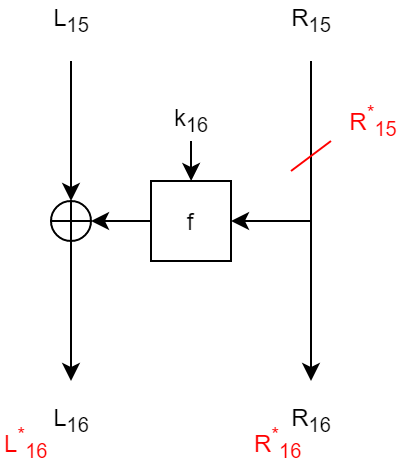
\includegraphics[scale=0.4]{DES_atq.png}\end{center}
		
		Pour exploiter cette faute, on va analyser les résultats obtenus à la sortie du 16\up{ème} tour. On a :
		\begin{itemize}
			\item $L_{16} = L_{15} \oplus f(R_{15}, k_{16})$
			\item $R_{16} = R_{15}$
			\item $L_{16}^{*} = L_{15} \oplus f(R_{15}^{*}, k_{16})$
			\item $L_{16}^{*} = R_{15}^{*}$
		\end{itemize}
		
		On remarque que $L_{16}$ et $L_{16}^{*}$ font toutes les deux intervenir la clé $k_{16}$ qui est l'objet initial de cette attaque. On exploite donc $L_{16}$ et $L_{16}^{*}$ pour construire une équation permettant de retrouver $k_{16}$. On effectue un XOR entre $L_{16}$ et $L_{16}^{*}$ pour éliminer $L_{15}$, l'équation obtenue est donc :
		\[L_{16} \oplus L_{16}^{*} = f(R_{15}, k_{16}) \oplus f(R_{15}^{*}, k_{16}) \]
		
		On va maintenant s'intéresser à la fonction interne $f$ du DES afin de mieux exploiter l'équation obtenue précédemment. Cette fonction est illustrée par la figure ci-dessous :
		
		\begin{center}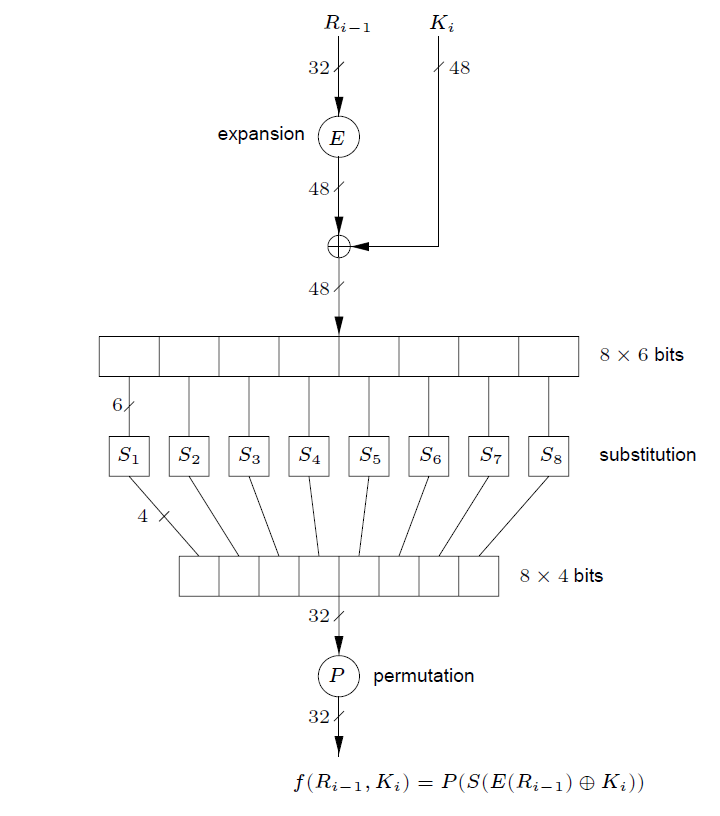
\includegraphics[scale=0.7]{DES_f.png}\end{center}
		
		L'analyse de cette fonction nous permet d'établir que :
		\begin{itemize}
			\item $f(R_{15}, k_{16}) \ = \ P\ [ \quad S_{1}({E(R_{15}) \oplus k_{16}}_{\ \textrm{bits}\ 1 \to 6}) \quad ||\ ...\ || \quad S_{8}({E(R_{15}) \oplus k_{16}}_{\ \textrm{bits}\ 43 \to 48}) \quad ]$			
			\item $f(R_{15}^{*}, k_{16}) \ = \ P\ [ \quad S_{1}({E(R_{15}^{*}) \oplus k_{16}}_{\ \textrm{bits}\ 1 \to 6}) \quad ||\ ...\ || \quad S_{8}({E(R_{15}^{*}) \oplus k_{16}}_{\ \textrm{bits}\ 43 \to 48}) \quad ]$
		\end{itemize}
		
		En effet, la fonction $f$ prend en entré le demi-bloc $R$ de 32 bits auquel elle applique une expansion de 48 bits, ainsi que la clé $k_{16}$. Ces deux entrées sont mélangées à l'aide d'un XOR pour obtenir une entité de 48 bits. Ces 48 bits vont être répartis sur 8 boites de substitution appelées \textit{S-box}. Chacune des 8 S-box prend 6 bits en entrée et en renvoie 4, pour avoir un résultat final de 32 bits. Ces S-box vont être l'objet principal de l'attaque. L'équation précédemment établie devient ainsi :
		\[L_{16} \oplus L_{16}^{*} = f(R_{15}, k_{16}) \oplus f(R_{15}^{*}, k_{16}) \]
		\[\Leftrightarrow\]		
		\[L_{16} \oplus L_{16}^{*}\]
		\[=\] 
		\[P\ [\ S_{1}({E(R_{15}) \oplus k_{16}}_{\ \textrm{bits}\ 1 \to 6}) \quad ||\ ...\ || \quad S_{8}({E(R_{15}) \oplus k_{16}}_{\ \textrm{bits}\ 43 \to 48})\ ] \]
		\[\oplus\] 
		\[P\ [\ S_{1}({E(R_{15}^{*}) \oplus k_{16}}_{\ \textrm{bits}\ 1 \to 6}) \quad ||\ ...\ || \quad S_{8}({E(R_{15}^{*}) \oplus k_{16}}_{\ \textrm{bits}\ 43 \to 48})\ ] \]
		
		\noindent En appliquant l'inverse de la permutation P (calculée à la main en prenant le chemin inverse de la permutation P fournie dans la documentation du DES), et en s'appuyant la propriété d'une permutation P quelconque, $P(a \oplus b) = P(a) \oplus P(b)$, on obtient :
		\[P^{-1}(L_{16} \oplus L_{16}^{*})\]
		\[=\] 
		\[ S_{1}\ ({E(R_{15}) \oplus k_{16}}_{\ \textrm{bits}\ 1 \to 6})\quad \oplus \quad S_{1}\ ({E(R_{15}^{*}) \oplus k_{16}}_{\ \textrm{bits}\ 1 \to 6}) \]
		\[||\ ...\ ||\]
		\[ S_{8}\ ({E(R_{15}) \oplus k_{16}}_{\ \textrm{bits}\ 43 \to 48})\quad \oplus \quad S_{8}\ ({E(R_{15}^{*}) \oplus k_{16}}_{\ \textrm{bits}\ 43 \to 48}) \]
		\\
		\noindent Finalement, en répartissant cette équation sur les 8 S-box, on obtient 8 équations dont les membres font 4 bits et les solutions font 6 bits :
		\begin{itemize}
			\item $P^{-1}(L_{16} \oplus L_{16}^{*})_{\ \textrm{bits}\ 1 \to 4}\ = \ S_{1}\ (E(R_{15}) \oplus k_{16})_{\ \textrm{bits}\ 1 \to 4}\ \oplus \ S_{1}\ (E(R_{15}^{*}) \oplus k_{16})_{\ \textrm{bits}\ 1 \to 4}$
			\item ...
			\item $P^{-1}(L_{16} \oplus L_{16}^{*})_{\ \textrm{bits}\ 29 \to 32}\ = \ S_{8}\ (E(R_{15}) \oplus k_{16})_{\ \textrm{bits}\ 29 \to 32}\ \oplus \ S_{8}\ (E(R_{15}^{*}) \oplus k_{16})_{\ \textrm{bits}\ 29 \to 32}$
		\end{itemize}
		
		La seule inconnue dans toutes ces équations est $k_{16}$. Pour trouver $k_{16}$, il faut faire une recherche exhaustive sur chacune des 8 S-box correspondant à chacune des 8 équations. Chaque recherche sur les S-box va permettre de révéler 6 bits de $k_{16}$, pour en avoir au final 48 bits. La complexité de cette attaque est donc de $8$ x $2^{6}$.
		
	\section*{Question 2}
		\subsection*{2.1 Recherche de la clé $k_{16}$ de 48 bits}
		\noindent \underline{Remarque :} les manipulations décrites dans cette partie sont implémentées dans le fichier source \lstinline!DES_K16.c!.
		
\end{document}
